% \iffalse
\let\negmedspace\undefined
\let\negthickspace\undefined
\documentclass[journal,12pt,twocolumn]{IEEEtran}
\usepackage{cite}
\usepackage{amsmath,amssymb,amsfonts,amsthm}
\usepackage{algorithmic}
\usepackage{graphicx}
\usepackage{textcomp}
\usepackage{xcolor}
\usepackage{txfonts}
\usepackage{listings}
\usepackage{enumitem}
\usepackage{mathtools}
\usepackage{gensymb}
\usepackage{comment}
\usepackage[breaklinks=true]{hyperref}
\usepackage{tkz-euclide}
\usepackage{listings}
\usepackage{gvv}
\def\inputGnumericTable{}
\usepackage[latin1]{inputenc}
\usepackage{color}
\usepackage{array}
\usepackage{longtable}
\usepackage{calc}
\usepackage{multirow}
\usepackage{hhline}
\usepackage{ifthen}
\usepackage{lscape}

\newtheorem{theorem}{Theorem}[section]
\newtheorem{problem}{Problem}
\newtheorem{proposition}{Proposition}[section]
\newtheorem{lemma}{Lemma}[section]
\newtheorem{corollary}[theorem]{Corollary}
\newtheorem{example}{Example}[section]
\newtheorem{definition}[problem]{Definition}
\newcommand{\BEQA}{\begin{eqnarray}}
\newcommand{\EEQA}{\end{eqnarray}}
\newcommand{\define}{\stackrel{\triangle}{=}}
\theoremstyle{remark}
\newtheorem{rem}{Remark}
\begin{document}

\bibliographystyle{IEEEtran}
\vspace{3cm}

\title{NCERT Discrete - 10.5.2.19}
\author{EE23BTECH11007 - Aneesh Kadiyala$^{*}$% <-this % stops a space
}
\maketitle
\newpage
\bigskip

\renewcommand{\thefigure}{\theenumi}
\renewcommand{\thetable}{\theenumi}
%fi

\vspace{3cm}
\textbf{Question 10.5.2.19:} Subba Rao started work in 1995 at an annual salary of Rs. 5000 and received an increment of Rs. 200 each year. In which year did his income reach Rs. 7000?
\\
\solution
\begin{table}[h!]
    \centering
    \caption{Input Parameters}
    \label{tab:1}
    \begin{tabular}{ | c | c | c | }
        \hline
        Parameter & Value & Description \\
        \hline
        $x(0)$ & 5000 & Initial Income \\
        \hline
        $d$ & 200 & Annual Increment (Common Difference) \\
        \hline
        $x(n)$ & $x(0) + nd$ & $n^{th}$ term of the AP \\
        \hline
    \end{tabular}
\end{table}
\begin{align}
7000 &= 5000 + (n - 1)(200) \\
2000 &= (n - 1)(200) \\
n &= 11
\end{align}

\begin{enumerate}
\item Finding $x(n)$

The series is an arithmetic progression.
\begin{align}
x(n) = x(0) + nd
\end{align}

From \tabref{tab:1}:
\begin{align}
x(n) = (5000 + 200n)(u(n))
\end{align}
as $x(n) = 0 \forall n < 0$.

\begin{figure}[h!]
    \centering
    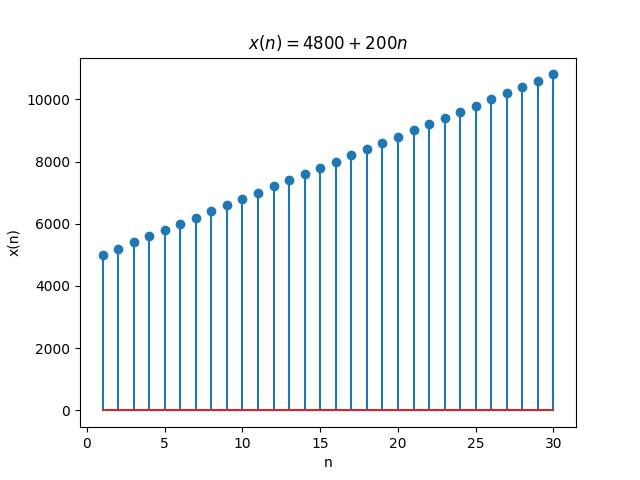
\includegraphics[width=\columnwidth]{figs/10_5_2_19.png}
    \caption{Plot of $x(n)$ vs $n$}
    \label{fig:1}
\end{figure}

\item Z-transform of $x(n)$ \\
Let Z-transform of $x(n)$ be $X(z)$. Let U(z) be the Z-transform of $u(n)$.
\begin{align}
X(z) &= \sum_{n = -\infty}^{\infty} (5000 + 200n)(u(n))(z^{-n}) \\
X(z) &= 5000\sum_{n = -\infty}^{\infty} u(n)(z^{-n}) + 200\sum_{n = -\infty}^{\infty}n(u(n))(z^{-n})
\end{align}
Using differentiation in Z-domain property,
\begin{align}
Z\{nx(n)\} &= -z\frac{d}{dz}X(z) \\
X(z) &= 5000U(z) + 200(-z)\frac{d}{dz} U(z) \\
&= \frac{5000}{1 - z^{-1}} + 200(-z)(-\frac{1}{z^2(1 -z^{^-1})^2}) \\
&= 5000(1 - z^{-1})^{-1} + 200\frac{z}{(z - 1)^2} \\
X(z) &= \frac{5000z}{z - 1} + \frac{200z}{(z - 1)^2} \forall |z| > 1
\end{align}

\end{enumerate}
\end{document}